\\\;
\\{\Large Kmeans Algorithm}
\\ well, firstly we import required libraries, then reading data and drawing a scatter plot to have a broad overview of how data looks like.
 as we can see there are five crowds(just like we we've been asked) and then we wish to split these clusters in the end of this process.

\begin{landscape}
\vspace*{0cm}
\hspace*{-0.5cm}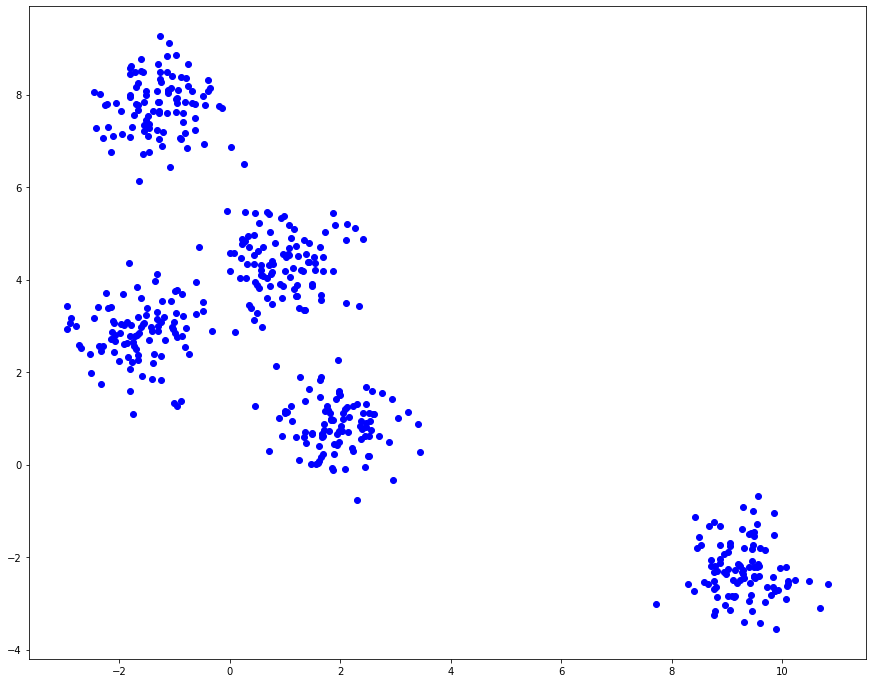
\includegraphics[width = 1 \linewidth]{scatter.png}
\hspace*{2cm}
\end{landscape}
\\it seems like best distance we could work with is Euclidean(L2 norm)and so we do!
\\finally we are so good to start our algorithm 
\\\indent define our parameters
\\\indent making our starting point through the way commented in the code
\\\indent and starting the main "for" loop
\\ Distance matrix (Dist) has diatance of points from means in columns 1:5 and from zero in column 0 and "which" is list which says which mean point is the closest for each datapoint.
\\assigning datapoints to their corresponding clusters with the help of "which" and we have our first cluster!
\\finally meanpoints would get updated (they're in the middle of their cluster) and doing the loop over and over to see better resuls 

\begin{landscape}
\vspace*{0cm}
\hspace*{-0.5cm}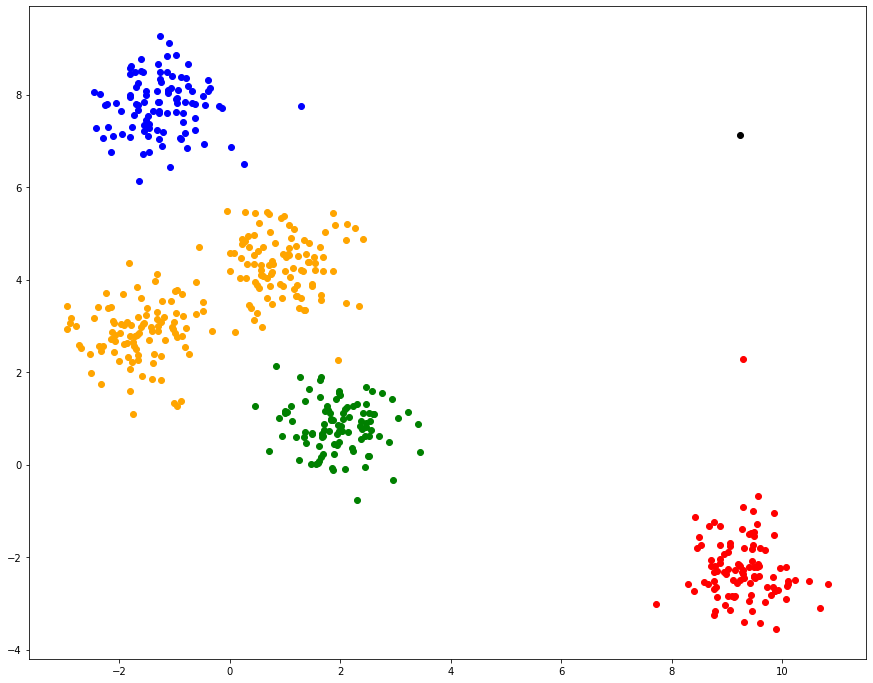
\includegraphics[width = 1 \linewidth]{clusters.png}
\hspace*{2cm}
\end{landscape}
\\it's not the desired clustering we had in mind, but thats all we could do.

\begin{landscape}
\vspace*{0cm}
\hspace*{-0.5cm}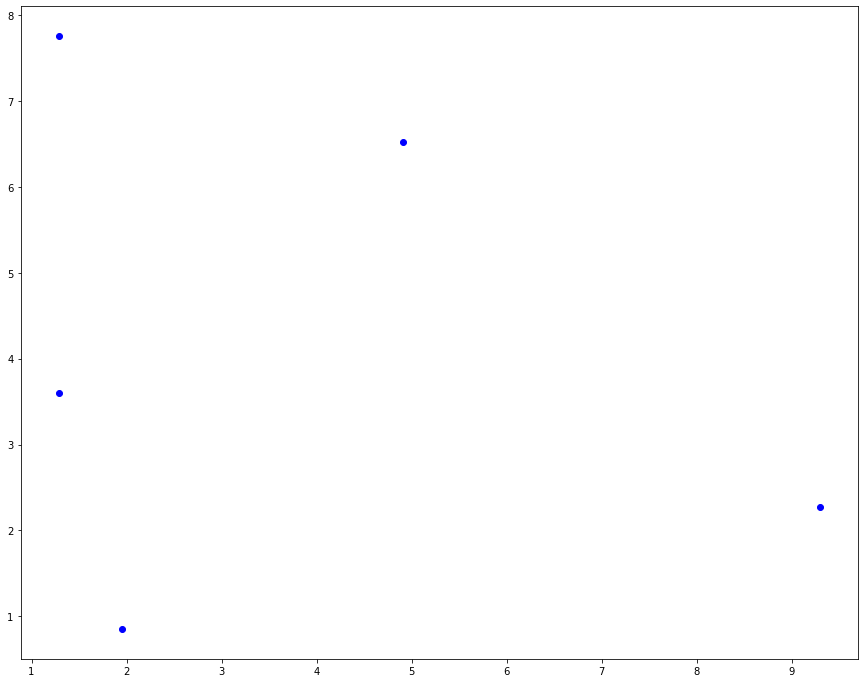
\includegraphics[width = 1 \linewidth]{means.png}
\hspace*{2cm}
\end{landscape}

\\and these are the mean points which clusters are formed around them
\\\;
\\\;
\\\textbf{Thanke you}
